\ifnum \Solutions=1 \newpage \fi

\ifnum \Version = 4
\question[2] Suppose $A = \begin{pmatrix} 4&1\\8&2 \end{pmatrix}$. On the grids below, sketch a) $\Null A$ and b) $(\Col A)^{\perp}$. You do not need to show your work. 


\ifnum \Solutions=1 {\color{DarkBlue} \textit{Solutions.} \begin{itemize}
    \item[a)] The null space is the set of all solutions to $Ax=0$, which we could find by row reducing the augmented matrix $(A \, | \, 0)$: \begin{align}
    (A \, | \, 0) = \begin{pmatrix} 4&1&0\\8&2&0 \end{pmatrix} \sim \begin{pmatrix} 4&1&0\\0&0&0 \end{pmatrix}
\end{align} The first row is $4x_1 + x_2 = 0$. So if $x_1=1$, then $x_2=-4$. So, we sketch the line that passes through the origin and the point $(1,-4)$. Note also that the span is a line that is defined for any value of $x_1$. So to sketch the span correctly, the line needs to extend to the edges of the graph. 
\item[b)] Remember that $(\Col A)^{\perp} = \Null (A^T)$. And $A^T = \begin{pmatrix} 4&8\\1&2\end{pmatrix}$. To determine the null space of $A^T$ we can row reduce the augmented matrix $(A^T \, | \, 0)$: \begin{align}
    (A \, | \, 0) = \begin{pmatrix} 4&8&0\\1&2&0 \end{pmatrix} \sim \begin{pmatrix} 1&2&0\\0&0&0 \end{pmatrix}
\end{align} The first row is $x_1 + 2x_2 = 0$. So if $x_1=2$, then $x_2=-1$. So, we sketch the line that passes through the origin and the point $(2,-1)$. Note also that the span is a line that is defined for any value of $x_1$. So to sketch the span correctly, the line needs to extend to the edges of the graph. 
\end{itemize}
    \vspace{-12pt}
    \begin{center}
    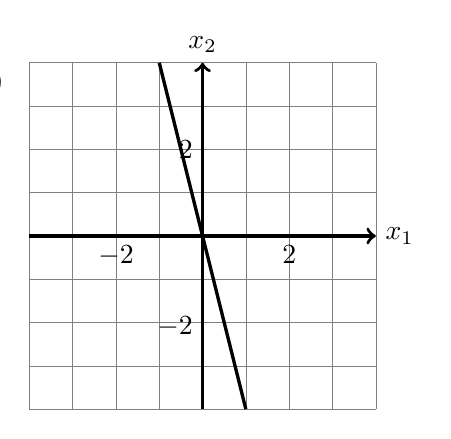
\begin{tikzpicture}[scale=.55]
    \draw[help lines] (-4, -4) grid (4, 4);
\draw[very thick, ->] (-4, 0) -- (4, 0);
\draw[very thick, ->] (0, -4) -- (0, 4);
\node[above] at (0, 4) {$x_2$};
\node[right] at (4, 0) {$x_1$};
\node[left] at (0, 2) {$2$};
\node[below] at (2, 0) {$2$};
\node[below] at (-2, 0) {$-2$};
\node[left] at (0, -2.1) {$-2$};    
    \node[overlay, above] at (-5, 3) {(a)};
    \draw[very thick, -] (1, -4) -- (-1, 4);    
    \end{tikzpicture}\qquad
    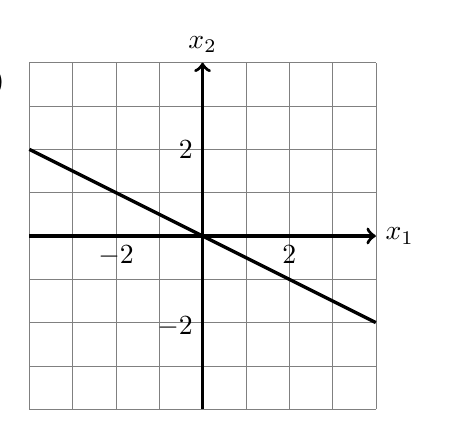
\begin{tikzpicture}[scale=.55]
    \draw[help lines] (-4, -4) grid (4, 4);
\draw[very thick, ->] (-4, 0) -- (4, 0);
\draw[very thick, ->] (0, -4) -- (0, 4);
\node[above] at (0, 4) {$x_2$};
\node[right] at (4, 0) {$x_1$};
\node[left] at (0, 2) {$2$};
\node[below] at (2, 0) {$2$};
\node[below] at (-2, 0) {$-2$};
\node[left] at (0, -2.1) {$-2$};    
    \node[overlay, above] at (-5, 3) {(b)};  
    \draw[very thick, -] (4, -2) -- (-4, 2);    
    \end{tikzpicture}
    \end{center}   }
   \else
    \vspace{-12pt}
    \begin{center}
    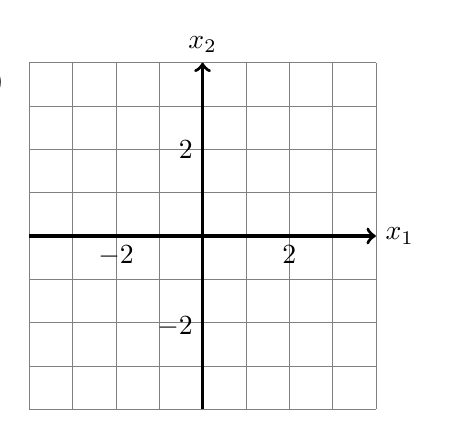
\begin{tikzpicture}[scale=.55]
    \draw[help lines] (-4, -4) grid (4, 4);
\draw[very thick, ->] (-4, 0) -- (4, 0);
\draw[very thick, ->] (0, -4) -- (0, 4);
\node[above] at (0, 4) {$x_2$};
\node[right] at (4, 0) {$x_1$};
\node[left] at (0, 2) {$2$};
\node[below] at (2, 0) {$2$};
\node[below] at (-2, 0) {$-2$};
\node[left] at (0, -2.1) {$-2$};    
    \node[overlay, above] at (-5, 3) {(a)};
    \end{tikzpicture}\qquad
    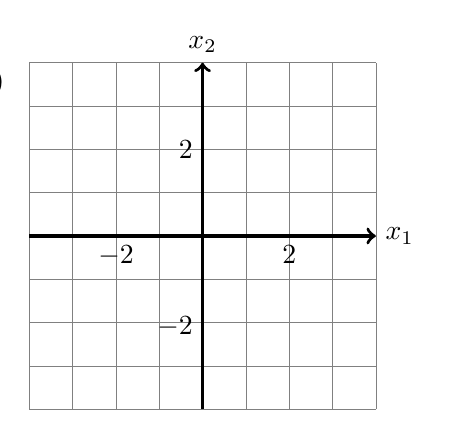
\begin{tikzpicture}[scale=.55]
    \draw[help lines] (-4, -4) grid (4, 4);
\draw[very thick, ->] (-4, 0) -- (4, 0);
\draw[very thick, ->] (0, -4) -- (0, 4);
\node[above] at (0, 4) {$x_2$};
\node[right] at (4, 0) {$x_1$};
\node[left] at (0, 2) {$2$};
\node[below] at (2, 0) {$2$};
\node[below] at (-2, 0) {$-2$};
\node[left] at (0, -2.1) {$-2$};    
    \node[overlay, above] at (-5, 3) {(b)};    
    \end{tikzpicture}
    \end{center}   
   \fi
\fi



\ifnum \Version = 11
\question[2] Construct an orthogonal basis for $W = \text{Span}\{v_1,v_2\}$. Please show your work. 
$$v_1 = \begin{pmatrix} 1\\1\\1\end{pmatrix}, \quad v_2 = \begin{pmatrix} 3\\5\\1\end{pmatrix}$$

\ifnum \Solutions=1 {\color{DarkBlue} \textit{Solutions.} Set $\hat v_1 = v_1$ and $\hat v_2$ to be
$$\hat v_2 = v_2 - \frac{v_1\cdot v_2}{v_1\cdot v_1} v_1 = \begin{pmatrix} 3\\5\\1\end{pmatrix} - \frac{9}{3}\begin{pmatrix} 1\\1\\1\end{pmatrix} = \begin{pmatrix} 0\\2\\-2\end{pmatrix}$$ An orthogonal basis is $$\left\{ \begin{pmatrix}1\\1\\1 \end{pmatrix}, \begin{pmatrix} 0\\2\\-2\end{pmatrix}\right\}$$
}
\fi
\fi


\ifnum \Version = 12
\question[2] Suppose $A = \begin{pmatrix} 2&1\\8&4 \end{pmatrix}$. On the grids below, sketch a) the range of the transform $x \to Ax$, and b) $(\Row A)^{\perp}$. You do not need to show your work. 

\ifnum \Solutions=1 {\color{DarkBlue} \textit{Solutions.} \begin{itemize}
    \item[a)] The range is the span of the columns of $A$, and a vector in the span of the columns is $\begin{pmatrix} 1 & 4\end{pmatrix}^T$. We can sketch a line that passes through the origin and the point $(1,4)$. Note also that the span is a line that is defined for any value of $x_1$. So to sketch the span correctly, the line needs to extend to the edges of the graph. 
    \item[b)] Remember that $(\Row A)^{\perp} = \Null A$. The rows are dependent, so we can ignore one of the rows and use the other to sketch the space. For example we can sketch the line that passes through the origin and the point $(2,-1)$. Note also that the span is a line that is defined for any value of $x_1$. So to sketch the span correctly, the line needs to extend to the edges of the graph. 
    \end{itemize}
    \vspace{-12pt}
    \begin{center}
    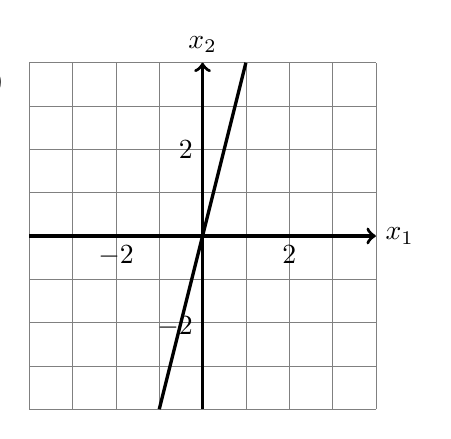
\begin{tikzpicture}[scale=.55]
    \draw[help lines] (-4, -4) grid (4, 4);
\draw[very thick, ->] (-4, 0) -- (4, 0);
\draw[very thick, ->] (0, -4) -- (0, 4);
\node[above] at (0, 4) {$x_2$};
\node[right] at (4, 0) {$x_1$};
\node[left] at (0, 2) {$2$};
\node[below] at (2, 0) {$2$};
\node[below] at (-2, 0) {$-2$};
\node[left] at (0, -2.1) {$-2$};    
    \node[overlay, above] at (-5, 3) {(a)};
    \draw[very thick, -] (-1,-4) -- (1,4);    
    \end{tikzpicture}\qquad
    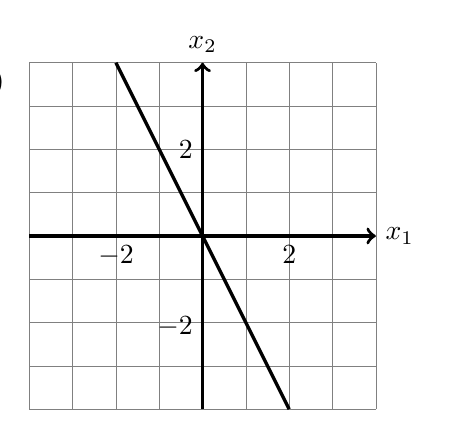
\begin{tikzpicture}[scale=.55]
    \draw[help lines] (-4, -4) grid (4, 4);
\draw[very thick, ->] (-4, 0) -- (4, 0);
\draw[very thick, ->] (0, -4) -- (0, 4);
\node[above] at (0, 4) {$x_2$};
\node[right] at (4, 0) {$x_1$};
\node[left] at (0, 2) {$2$};
\node[below] at (2, 0) {$2$};
\node[below] at (-2, 0) {$-2$};
\node[left] at (0, -2.1) {$-2$};    
    \node[overlay, above] at (-5, 3) {(b)};  
    \draw[very thick, -] (-2, 4) -- (2, -4);    
    \end{tikzpicture}
    \end{center}   }
   \else
    \vspace{-12pt}
    \begin{center}
    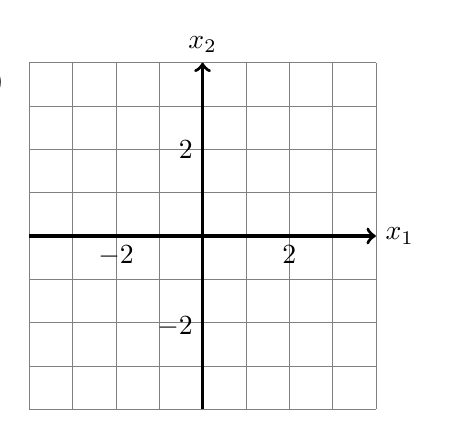
\begin{tikzpicture}[scale=.55]
    \draw[help lines] (-4, -4) grid (4, 4);
\draw[very thick, ->] (-4, 0) -- (4, 0);
\draw[very thick, ->] (0, -4) -- (0, 4);
\node[above] at (0, 4) {$x_2$};
\node[right] at (4, 0) {$x_1$};
\node[left] at (0, 2) {$2$};
\node[below] at (2, 0) {$2$};
\node[below] at (-2, 0) {$-2$};
\node[left] at (0, -2.1) {$-2$};    
    \node[overlay, above] at (-5, 3) {(a)};
    \end{tikzpicture}\qquad
    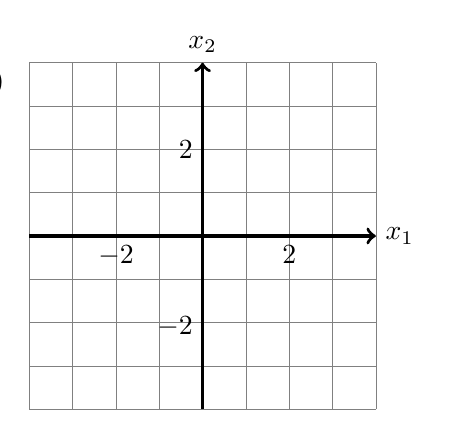
\begin{tikzpicture}[scale=.55]
    \draw[help lines] (-4, -4) grid (4, 4);
\draw[very thick, ->] (-4, 0) -- (4, 0);
\draw[very thick, ->] (0, -4) -- (0, 4);
\node[above] at (0, 4) {$x_2$};
\node[right] at (4, 0) {$x_1$};
\node[left] at (0, 2) {$2$};
\node[below] at (2, 0) {$2$};
\node[below] at (-2, 0) {$-2$};
\node[left] at (0, -2.1) {$-2$};    
    \node[overlay, above] at (-5, 3) {(b)};    
    \end{tikzpicture}
    \end{center}   
   \fi
\fi



\ifnum \Version = 13
\question[2] Suppose $A = \begin{pmatrix} 4&1\\8&2 \end{pmatrix}$. On the grids below, sketch a) the eigenspace corresponding to eigenvalue $\lambda = 6$, and b) $(\Null A)^{\perp}$. You do not need to show your work. 


\ifnum \Solutions=1 {\color{DarkBlue} \textit{Solutions.} \begin{itemize}
    \item[a)] The eigenspace is the space spanned by vectors in $\Null(A - \lambda I)$. $$A - \lambda I = \begin{pmatrix}-2&1\\8&-4 \end{pmatrix}$$ A vector in the nullspace is the eigenvector $v = \begin{pmatrix} 1\\2\end{pmatrix}$. We can sketch a line that passes through the origin and the point $(1,2)$. Note also that the span is a line that is defined for any value of $x_1$. So to sketch the span correctly, the line needs to extend to the edges of the graph. 
\item[b)] Remember that $(\Null A)^{\perp} = \Row A$. The rows are dependent, so we can ignore one of the rows and use the other to sketch the space. For example we can sketch the line that passes through the origin and the point $(4,1)$. Note also that the span is a line that is defined for any value of $x_1$. So to sketch the span correctly, the line needs to extend to the edges of the graph. 
\end{itemize}
    \vspace{-12pt}
    \begin{center}
    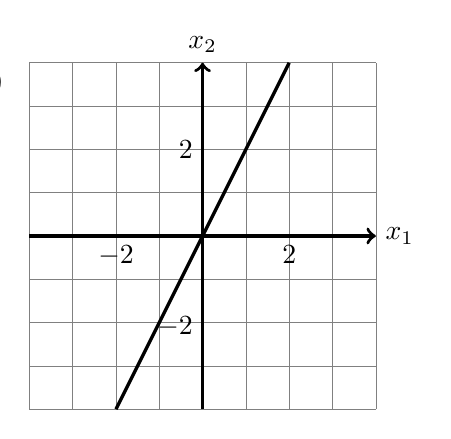
\begin{tikzpicture}[scale=.55]
    \draw[help lines] (-4, -4) grid (4, 4);
\draw[very thick, ->] (-4, 0) -- (4, 0);
\draw[very thick, ->] (0, -4) -- (0, 4);
\node[above] at (0, 4) {$x_2$};
\node[right] at (4, 0) {$x_1$};
\node[left] at (0, 2) {$2$};
\node[below] at (2, 0) {$2$};
\node[below] at (-2, 0) {$-2$};
\node[left] at (0, -2.1) {$-2$};    
    \node[overlay, above] at (-5, 3) {(a)};
    \draw[very thick, -] (-2,-4) -- (2,4);    
    \end{tikzpicture}\qquad
    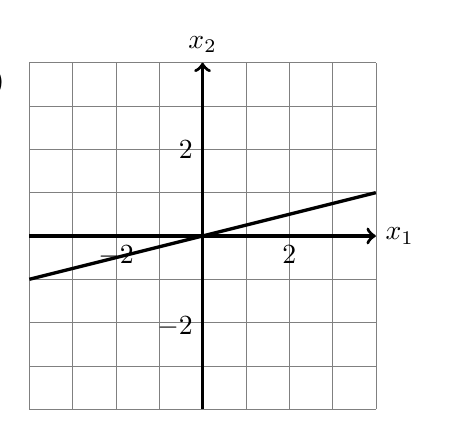
\begin{tikzpicture}[scale=.55]
    \draw[help lines] (-4, -4) grid (4, 4);
\draw[very thick, ->] (-4, 0) -- (4, 0);
\draw[very thick, ->] (0, -4) -- (0, 4);
\node[above] at (0, 4) {$x_2$};
\node[right] at (4, 0) {$x_1$};
\node[left] at (0, 2) {$2$};
\node[below] at (2, 0) {$2$};
\node[below] at (-2, 0) {$-2$};
\node[left] at (0, -2.1) {$-2$};    
    \node[overlay, above] at (-5, 3) {(b)};  
    \draw[very thick, -] (4, 1) -- (-4, -1);    
    \end{tikzpicture}
    \end{center}   }
   \else
    \vspace{-12pt}
    \begin{center}
    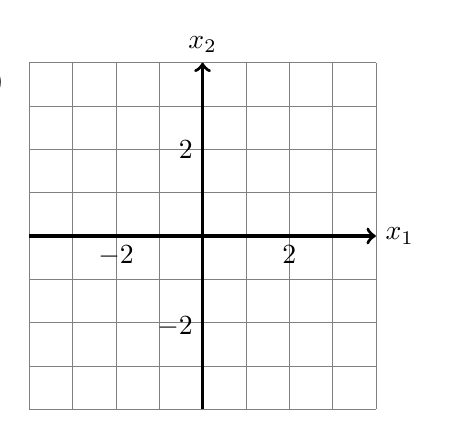
\begin{tikzpicture}[scale=.55]
    \draw[help lines] (-4, -4) grid (4, 4);
\draw[very thick, ->] (-4, 0) -- (4, 0);
\draw[very thick, ->] (0, -4) -- (0, 4);
\node[above] at (0, 4) {$x_2$};
\node[right] at (4, 0) {$x_1$};
\node[left] at (0, 2) {$2$};
\node[below] at (2, 0) {$2$};
\node[below] at (-2, 0) {$-2$};
\node[left] at (0, -2.1) {$-2$};    
    \node[overlay, above] at (-5, 3) {(a)};
    \end{tikzpicture}\qquad
    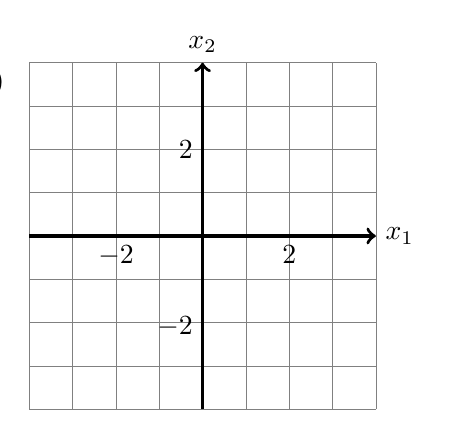
\begin{tikzpicture}[scale=.55]
    \draw[help lines] (-4, -4) grid (4, 4);
\draw[very thick, ->] (-4, 0) -- (4, 0);
\draw[very thick, ->] (0, -4) -- (0, 4);
\node[above] at (0, 4) {$x_2$};
\node[right] at (4, 0) {$x_1$};
\node[left] at (0, 2) {$2$};
\node[below] at (2, 0) {$2$};
\node[below] at (-2, 0) {$-2$};
\node[left] at (0, -2.1) {$-2$};    
    \node[overlay, above] at (-5, 3) {(b)};    
    \end{tikzpicture}
    \end{center}   
   \fi
\fi



\ifnum \Version = 20 %% NOT USING BUT COULD BE A GOOD QUESTION
\question[2] Construct an orthogonal basis for $W = \text{Span}\{v_1,v_2\}$. Please show your work. 
$$v_1 = \begin{pmatrix} 1\\1\\1\end{pmatrix}, \quad v_2 = \begin{pmatrix} 6\\10\\2\end{pmatrix}$$

\ifnum \Solutions=1 {\color{DarkBlue} \textit{Solutions.} NEED TO FIX THE SOLUTIONS THERE ARE SOME TYPOS HERE: Set $\hat v_1 = v_1$ and $\hat v_2$ to be
$$\hat v_2 = v_2 - \frac{v_1\cdot v_2}{v_1\cdot v_1} v_1 = \begin{pmatrix} 3\\5\\1\end{pmatrix} - \frac{18}{3}\begin{pmatrix} 1\\1\\1\end{pmatrix} = \begin{pmatrix} 3\\5\\1\end{pmatrix} -\begin{pmatrix} 6\\6\\6\end{pmatrix}= \begin{pmatrix}-3\\-1\\-5 \end{pmatrix}$$ An orthogonal basis is $$\left\{ \begin{pmatrix}1\\1\\1 \end{pmatrix}, \begin{pmatrix} 0\\2\\-2\end{pmatrix}\right\}$$
}
\fi
\fi